%% https://tipp2021.triumf.ca/proceedings.html
%% Deadline 25 June 2021
%% 4 page maximum
\documentclass[a4paper]{jpconf}
\usepackage{graphicx}
\usepackage{lineno}
\usepackage{subcaption}
\usepackage[utf8]{inputenc} % Включаем поддержку UTF8
\usepackage[russian,english]{babel}   % убрать русский перед отправкой статьи
\usepackage[pdftex, backref, colorlinks]{hyperref}
\usepackage{todonotes}
\pdfoutput=1 % if your are submitting a pdflatex (i.e. if you have
             % images in pdf, png or jpg format)

\graphicspath{{figures/}}
\bibliographystyle{iopart-num}

%%%%%%%%%%%%%%%%%%%%%%%%%%%%%%%%%%%%%%%%%%%%%%%%%
\begin{document}
\linenumbers % Remove after editing
\newcommand{\todoi}[1]{\todo[inline]{\Russian #1}}
%\tableofcontents  % пусть пока побудет, стереть перед подачей
%\listoftodos[NotesToDo]

\title{Status of the SPHERE project for the high energy cosmic ray study by registering reflected Cherenkov light with a drone-borne detector}

\author[1]{D.~Chernov$^{1,\ast}$, 
E.~Bonvech$^{1}$, 
M.~Finger~Jr.$^{2,3}$, 
M.~Finger$^{2,3}$,
V.~Galkin$^{1,4}$, 
V.~Ivanov$^{4}$, 
D.~Podgrudkov$^{1,4}$, 
T.~Roganova$^{1}$ 
and I.~Vaiman$^{1}$.}

\address{$^1$ Lomonosov Moscow State University, Skobeltsyn Institute for Nuclear Physics, Moscow, Russian Federation}
\address{$^2$ Charles University, Faculty of Mathematics and Physics, 18000 Prague, Czech Republic}
\address{$^3$ Joint Institute for Nuclear Research, Dubna, Russian Federation}
\address{$^4$ Lomonosov Moscow State University, Faculty of Physics, Moscow, Russian Federation}
% e-mail addresses: only for the corresponding author
\ead{chr@dec1.sinp.msu.ru}

%\keywords{Cherenkov detectors, balloon instrumentation, photon detectors for UV, visible and IR photons (Si-PMTs).}
%\arxivnumber{2005.07993} % only if you have one
%\proceeding{}

\begin{abstract}

Here we present the current status of the SPHERE project’s new detector technical design. The SPHERE project is aimed at the primary cosmic ray studies in 1-1000 PeV energy range using the reflected Cherenkov light method. The concept is discussed of a drone mounted detector with a photosensitive camera based on silicon photomultipliers. The design details of a small scale prototype of such a detector is presented.    
\end{abstract}


\section{Introduction}
\label{sec:intro}

%\todoi{Этот абзац почти повторяет текст предыдущей статьи}
%The energy range from 1 to 1000 PeV is a transitional one from galactic to extragalactic primary cosmic rays (PCR). More than 50 years ago in this range near 3~PeV energy a change in slope of PCR energy spectrum was discovered. But the new features in energy spectrum structure are still being discovered. And the mechanisms and phenomena behind those features are of interest for present day astrophysics. One of the main reasons for those changes of slope most probably is the change in PCR mass composition. The existing method of PCR studies allows only the average PCR mass to be estimated or at best allows the division of the general PCR flux into separate `light' and `heavy' groups. In general, the PCR mass estimation is done using the comparison of data on average depth of extensive air shower (EAS) development maximum and the data of the cascade simulations.

The technique of the SPHERE project is based on the realization of proposed by Alexander Chudakov the primary cosmic ray study method~\cite{Chu74} of detection of the EAS Cherenkov light (CL) reflected from the snow ground surface. This technique was successfully implemented earlier in the SPHERE project\cite{Ant15a} in particular in the experiments with SPHERE-2 detector\cite{Ant20}. The small detector SPHERE-2 was carried by a tethered balloon above snow covered Baikal lake in Russia. The experiment was carefully simulated\cite{Ant19} and the results on the primary cosmic ray energy spectrum and the chemical composition were published\cite{Ant15c}. The event-by-event data analysis approach being an integral part of the reflected CL registration method allows higher accuracy in PCR mass composition study compared to existing ground detectors. This high accuracy is achieved through assigning a mass number to each individual event after a careful analysis of each EAS CL lateral distribution function without building any intermediate distribution of `typical' characteristics like depth of shower maximum. Now there are no detectors that have successfully used this technique.

The main aim of the current stage of the SPHERE project is to develop a new detector for PCR mass composition study in the energy range from 1 to 1000 PeV. The main advantage of the project is the use of silicon photomultipliers in a photosensitive camera and an unmanned aerial vehicle (UAV) to raise the detector above the ground. The combination of the method of recording reflected CL with its specific approaches to data analysis is a unique feature of this project.


\begin{figure}[t]
\centering % \begin{center}/\end{center} takes some additional vertical space
\begin{subfigure}[b]{0.45\textwidth}
    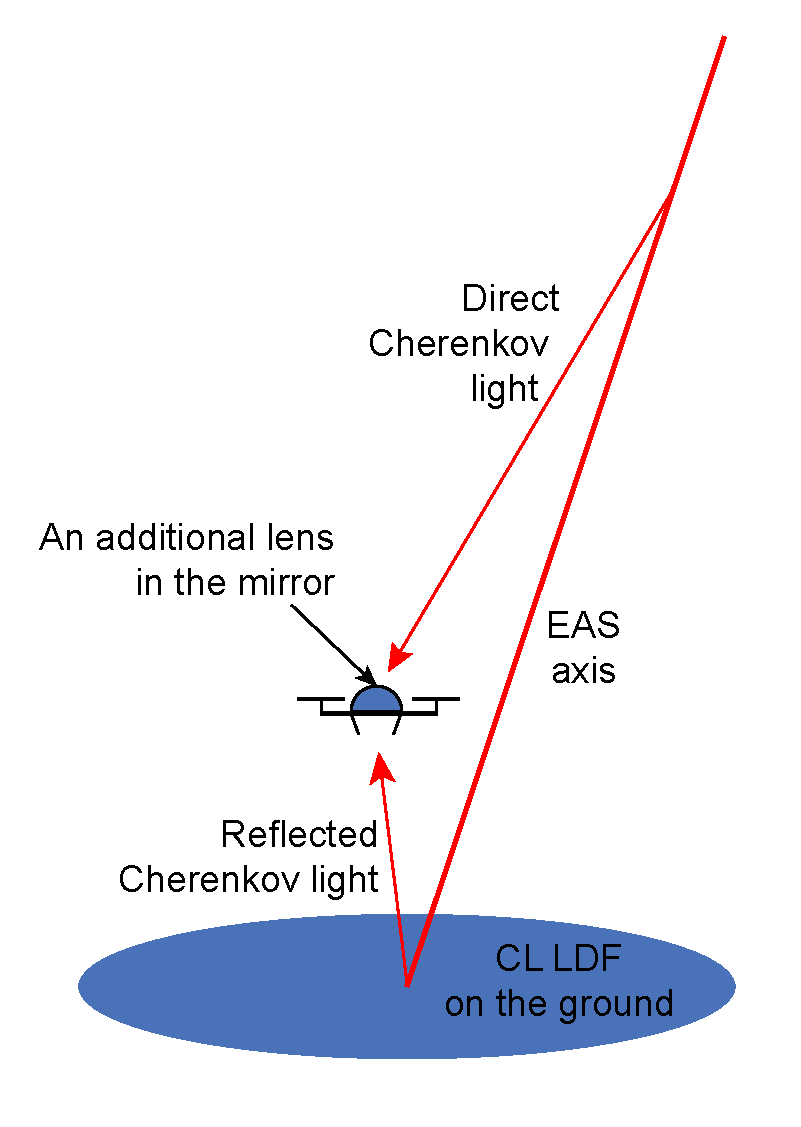
\includegraphics[height=.40\textheight]{DirectCL.pdf}
    \caption{Scheme of direct and reflected Cherenkov light of EAS.}
    \label{fig:DirectCL}
\end{subfigure}
\hfill
\begin{subfigure}[b]{0.53\textwidth}
%    \includegraphics[height=.25\textheight,trim = {11.5cm 0cm 0cm 0cm}, clip]{Sphere3optic.eps}}
    \includegraphics[height=.37\textheight, angle=-90]{Sphere3optic.eps}
    \includegraphics[height=.37\textheight, angle=-90]{Sphere3spot.eps}
    \caption{Preliminary version of the optical system with spot diagram analysis.}
    \label{fig:lightspots}
\end{subfigure}
\end{figure}

\begin{table}[tb]
\centering
\caption{Characteristics of the designing detectors.}
\label{tab:statistics}
%\vspace{1pc}
\begin{tabular}{| l |c|c|}
\hline
\textbf{Parameter}  & \parbox[t][.8cm]{3cm}{\textbf{Prototype of\\the detector}} & \textbf{Target Detector} \\ [1.5ex]
\hline
Sensitive area of optics (aperture input window) & 0,1 m$^2$ &  0.5 m$^2$\\ 
\hline
Mirror diameter & up to 80 cm &  up to 160 cm\\
\hline
Viewing angle of the optical system & $\pm$25$^\circ$ & $\pm$25$^\circ$ \\
\hline
Number of mosaic elements (silicon PMTs) & up to 133 & up to 3000 \\
\hline
Detector weight & up to 10 kg & up to 50 kg \\
\hline
Detector lifting height & up to 500 m & up to 2000 m \\
\hline
\end{tabular}
\end{table}


%\todoi{Этот текст повотряет текст предыдущей статьи}
%The method of reflected CL detection has the following advantages over traditional EAS detection methods:
%\begin{itemize}
%\item The method provides a significant area of CL detection using a compact device;
%\item Accurate estimation of PCR energy in an individual event thanks to the quasi-calorimetric method of energy detection;
%\item The field of view of individual sensitive elements of the device covers a significant part of the surveyed area, what allows to observe the EAS CL near the shower axis, usually inaccessible to ground-based CL detector arrays. This circumstance significantly increases the accuracy of the primary particle type estimation;
%\item Allows to measure the same PCR energy range with different resolution (distance between the centres of the fields of view of neighbouring sensory elements) by variating the elevation of the detector, thus allowing to control the magnitude of systematic errors;
%\item The small size of the required detector allows to combine the calibration techniques accessible currently only to imaging air Cherenkov telescopes (direct calibration) with large scale measurements that are accessible only for conventional ground-based arrays;
%\item Precise timing and high level of synchronization for better primary particle arrival direction reconstruction what has a direct impact on the precision of the EAS energy estimation.
%\item The compact and tight arrangement of the detector electronics and sensitive elements allows the use of complex local topological trigger conditions that can greatly decrease random coincidences thus allowing to lower the energy threshold for the measurements.
%\end{itemize}

\begin{figure}[t]
\centering % \begin{center}/\end{center} takes some additional vertical space
\includegraphics[width=0.38\textwidth]{Fig2_1.pdf}
\hfill
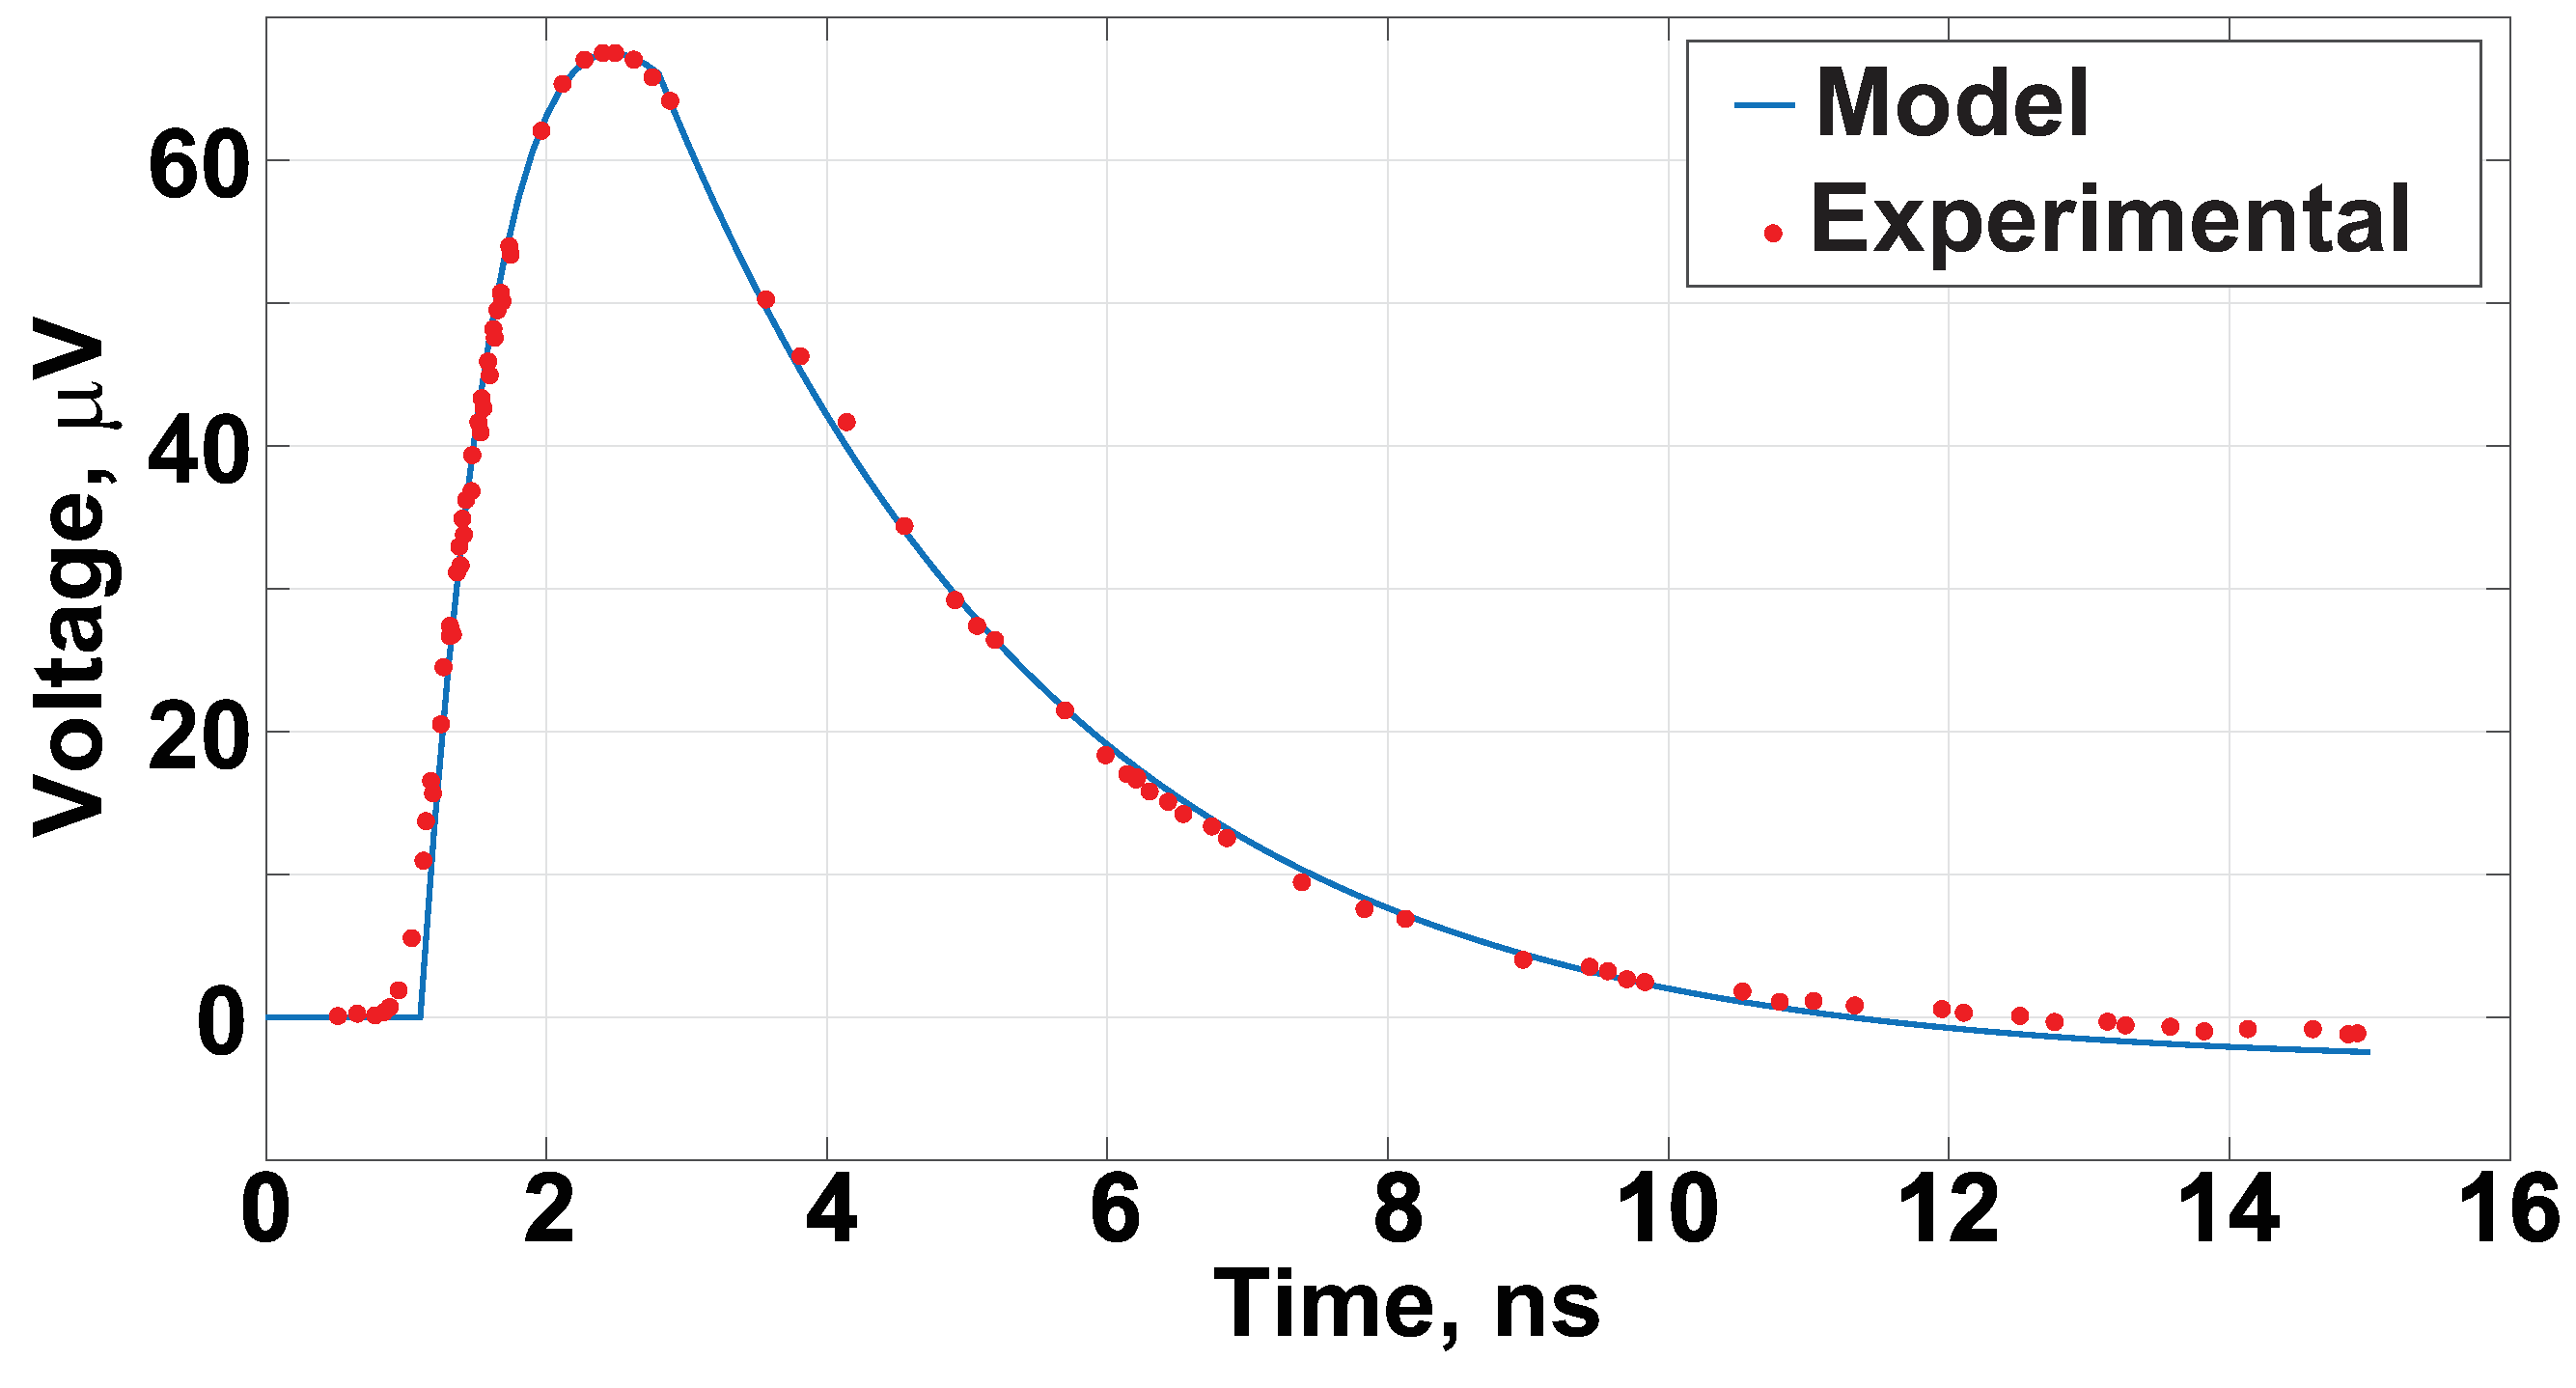
\includegraphics[width=0.60\textwidth]{Fig2_2.eps}
\caption{(Left) An electronic circuity model approximating real SiPM. The circuit model was built in MATLAB Simulink. (Right) The model curve of current pulse from a single photoelectron obtained from MATLAB Simulink in comparison to the manufacturer provided data.}
\label{fig:Sphere_results}
\end{figure}


\section{Detector Design}

%На рисунке 1b приведена предварительная схема оптической системы для прототипа детектора. Угол обзора детектора составляет $pm$25$^\circ$. При диаметре зеркала 800мм и диаметре входного окна диафрагмы 460мм размер светового пятна на мозаике SiPM составляет около 20мм. Характеристики оптических систем разрабатываемого детектора и его прототипа приведены в таблице \ref{tab:statistics}.

Since the detector will use the Schmidt optical system. In this system, the central part of the mirror is not used since it is in the shadow of the photodetector. This area can be used by a system with approximate aperture of 100 cm$^2$ for registration of the direct CL. Calculations show that for the EAS from 1 PeV proton the CL photons density is ~100 photons per cm at a distance of 100 m from the shower axis. Taking into account the SiPM quantum efficiency and losses on optical elements the expected number of registered photoelectrons is around 1000. The estimation of the primary particle mass can use the information on the intensity and angular properties of the direct CL in addition to the data on the reflected CL. It is assumed that the EAS from the primary proton should form a light spot different of Fe nuclei at the same primary energy and depth of EAS maximum.

\subsection{SiPM segment prototype }
The main sensitive element of the new detector will consist of 7-channel SiPM boards[?,INSTR2020] based on Micro FC-60035 SiPMs~\cite{TunkaSIT2020}. The tests of a such boards were successfully completed. Each board was equipped with 7 preamplifiers and a temperature sensor. To increase the sensitivity of SiPM we plan to adapt the SiPM board for use in a wide angle optic based on hemispherical lenses.

\subsection{SiPM modelling}
% Для увеличения временного разрешения мы используем быстрый выход указанных выше SiPM. Однако, сигналы с этого выхода подвергаются искажениям в виде переколебания обратной полярности и наложения импульсов отдельных фотоэлектронов друг на друга. Для лучшего восстановления заряда сигналов мы повели моделирование работы SiPM c быстрым выодом. На рисунке 2 слева показана разработанная схема. Номиналы элементов схемы подобраны так чтобы смоделированный сигнал максимально правдоподобно описывал данные о форме измеренного импульса от производителя SiPM. На рисунке 2 справа показано хорошее соответствие откика модели SiPM и экспериментального импульса. 

\section{Experiment modeling}

\begin{figure}[t]
\centering % \begin{center}/\end{center} takes some additional vertical space
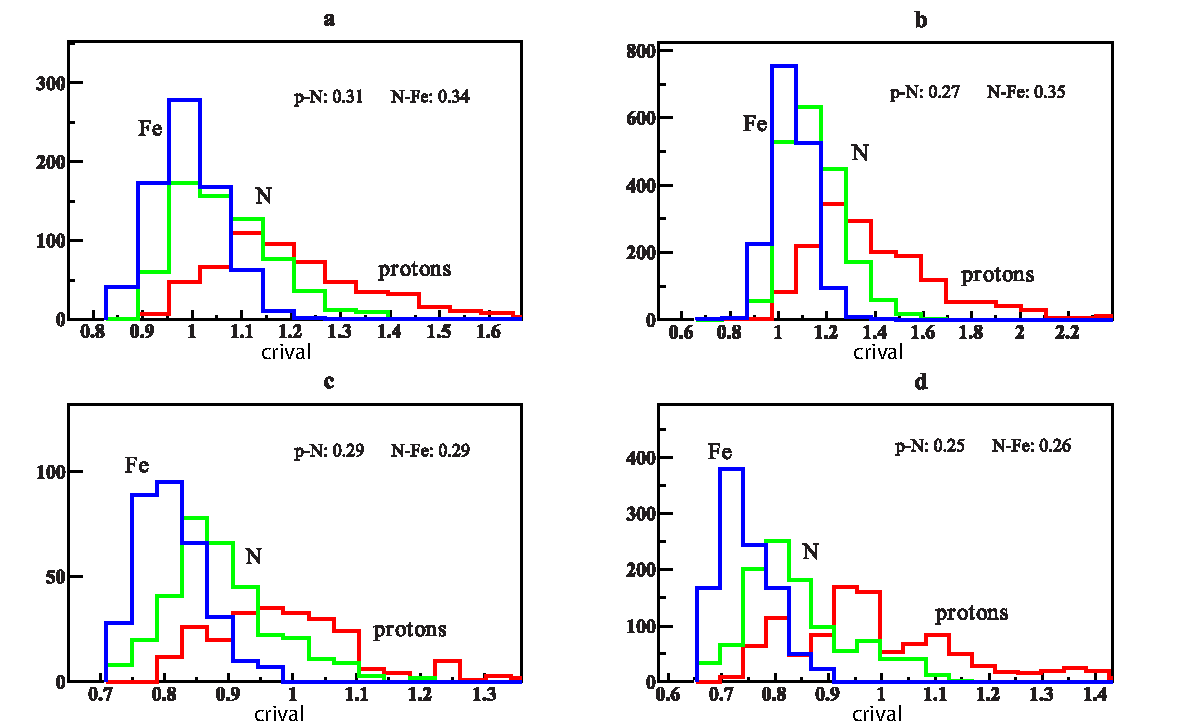
\includegraphics[width=\textwidth]{poster.pdf}
\caption{Criterion value distributions for p, N, Fe primaries. Zenith angle: $15^\circ$. Atmosphere model: 11. Figures inside the panels denote the probabilities of misclassification (classification errors) for pairs of primary particles p-N and N-Fe. \hspace{0.2cm}a,b -- $E_0$ = 10PeV, \hspace{0.2cm}c,d -- $E_0$ = 30PeV, \hspace{0.2cm}a,c -- h(elevation above the snowed surface) = 500m, \hspace{0.2cm}b,d -- h = 900m.}
\label{fig:Modelling}
\end{figure}

Modeling procedure generally follows the approach used in SPHERE-2 experiment. It includes event modeling and image processing.
Event modeling incorporates two stages: a) EAS simulation with CORSIKA code including Cherenkov light generation and b) the production of CL images of EAS events in the telescope mosaic. The 1st stage results in a detailed 3D-array of CL photoelecton distribution in coordinates and time delay on the snow for each EAS event. Photoelectons appear due to a special CORSIKA mode enabling account for the PMT efficiency during the shower modeling. At the 2nd stage the shower cores on the snow are evenly spread over a circle of 500 m radius centered under the telescope. Contributions to the mosaic PMTs from every patch of the CL spot on the snow are calculated on photoelectron-by-photoelectron basis.

While processing the images they are fitted with an axisymmetric rational function. Then the approximations are integrated over a central circle and the surrounding ring. Ratio of these integrals is used as a criterion parameter for the separation of events by the primary mass. Criteria are optimized with respect to the mass separation by varying the radii of the circle and the ring. Optimal criteria are obtained for different primary energies and zenith angles, detector elevation and atmosphere models (1 and 11 in CORSIKA terms).

Figure \ref{fig:Modelling} shows an example of primary mass criterion parameter distributions for p, N, Fe primaries made for SPHERE-2 detector, as the optical design of the new detector has not been completed.

The use of direct CL angular distribution will be considered as a possible means to enhance the EAS separation by the primary mass, which might help a lot in this matter, according to our previous developments\cite{Gal18a}.

%Criterion value distributions for p, N, Fe primaries. 

%Zenith angle: 15~$^\circ$. 
%Atmosphere model: 11. 

%Figures inside the panels denote the probabilities of misclassification (classification errors) for pairs of primary particles p-N and N-Fe.
%a,b --- $E_0$ = 10PeV, 
%c,d --- $E_0$ = 30PeV, 
%a,c --- $h$ (elevation above the snowed surface) = 500~m,
%b,d --- $h$ = 900~m.

\section{Conclusion}
The development of a new SiPM based detector for the EAS studied continues. A prototype of a photosensitive matrix element has been developed and is being tested. The detector design and feasibility of some technical solutions are being studied.  For this purpose, a SiPM circuit model with a fast output was created. The analysis of the detector design performance relative to the mass composition study is continued.

\section{Acknowledgments}
MEYS of Czech Republic grants LG14004 and LG18022.

\section*{References}
\bibliography{TIPP_Sphere}

\end{document}